% \newpage
% \begin{center}
%   \textbf{\large 5. Экспериментальное исследование разработанной двухотсчетной следящей системы}
% \end{center}
% \refstepcounter{chapter}
% \addcontentsline{toc}{chapter}{5. Экспериментальное исследование разработанной двухотсчетной следящей системы}


% \subsection{Структурная схема установки}
% Стенд (рис. \ref{STND-ISP}) представляет собой замкнутую электромеханическую систему, включающую:
% \begin{enumerate}
%     \item \textbf{Испытуемый модуль}: Блок АЦПВТ
%     \item \textbf{Отладочный двухканальный стенд}
%     \item \textbf{Эталонный измеритель}: Абсолютный энкодер Siemens 6FX2001-5HE25 
%     \item \textbf{Исполнительное устройство}: Асинхронный двигатель АИР56А4У3 
%     \item \textbf{Система управления}: Программируемый логический контроллер Siemens Sinamics S120
% \end{enumerate}

% \begin{figure}[!h]
%   \centering
%   \begin{subfigure}[b]{0.6\textwidth}
%     \centering
%     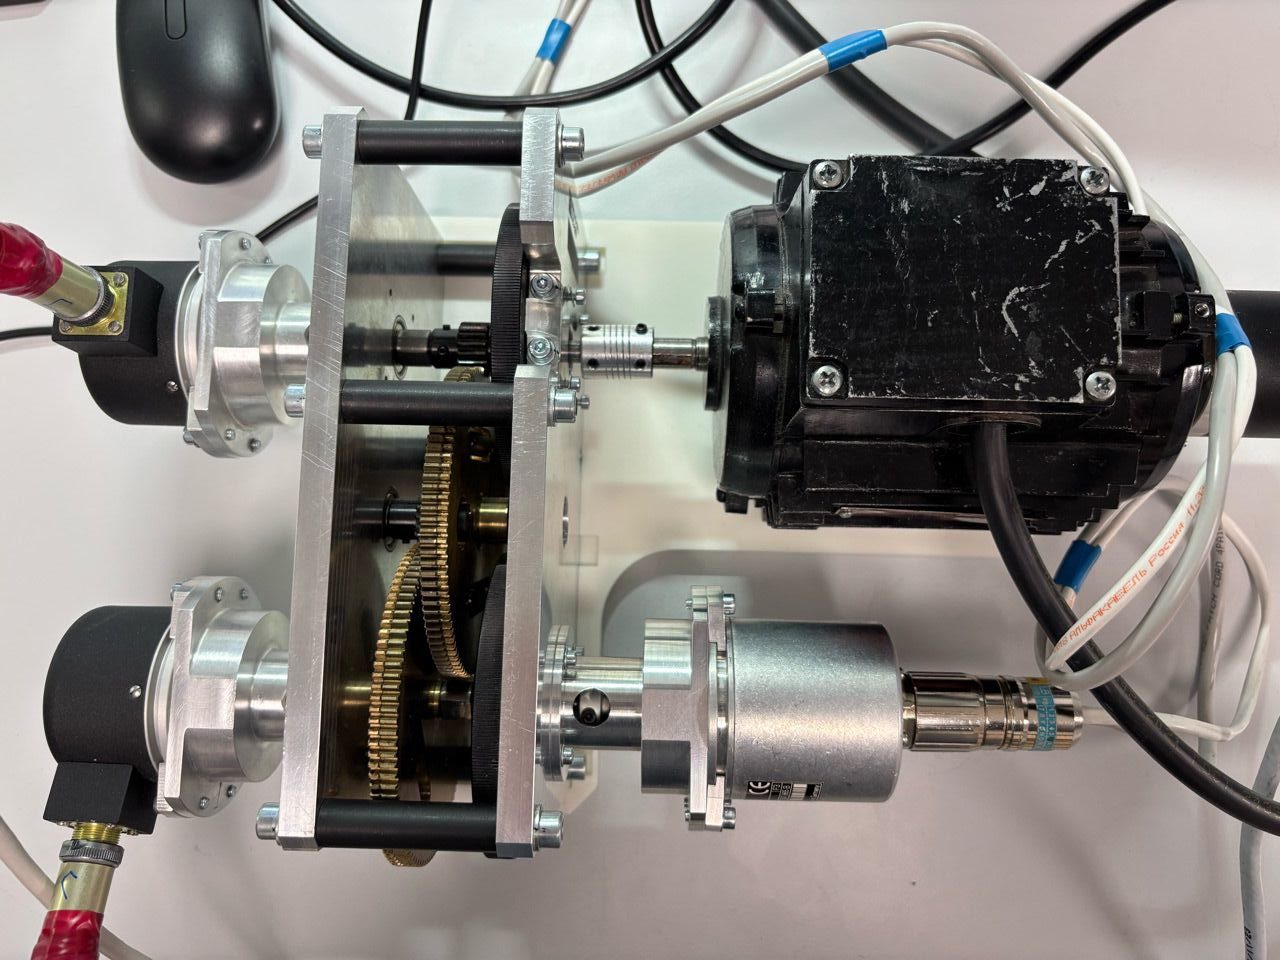
\includegraphics[width=\linewidth]{STND-01.jpg} 
%     \label{STND01}
%   \end{subfigure}
%   \hfill
%   \begin{subfigure}[b]{0.35\textwidth}
%     \centering
%     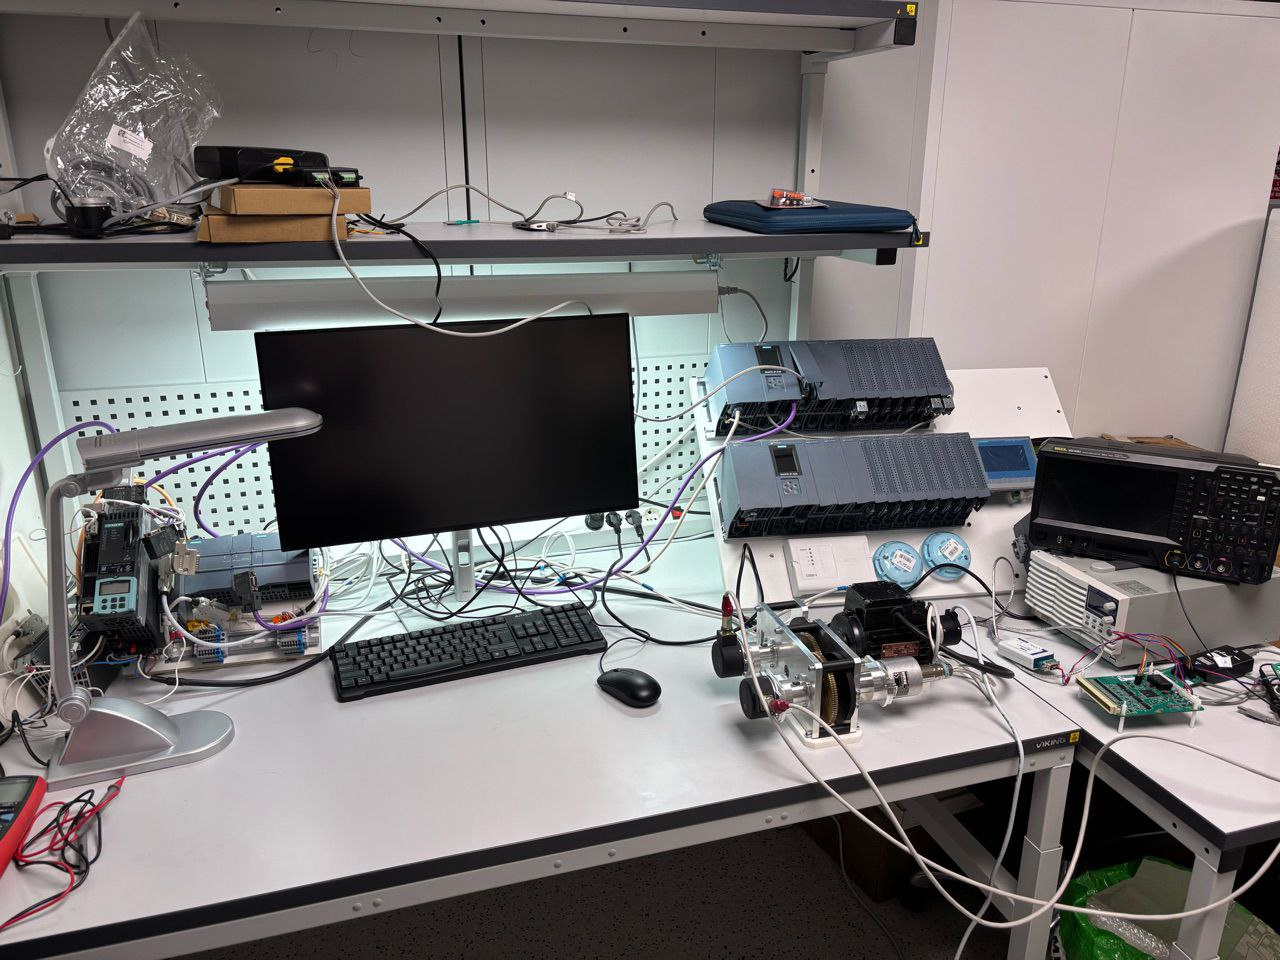
\includegraphics[width=\linewidth]{STND-02.jpg} 
%     \label{STND02}
%   \end{subfigure}

%   \caption{Испытательный стенд}
%   \label{STND-ISP} 
% \end{figure}



% \subsection{Методика проведения испытаний}
% Экспериментальные исследования включали три серии тестов:
% \begin{enumerate}
%     \item \textbf{Статическая точность}: Измерение погрешности при фиксированных углах с шагом $5^\circ$ в диапазоне $0^\circ-360^\circ$
%     \item \textbf{Динамические характеристики}: Анализ переходных процессов при угловых ускорениях и торможениях от $0^\circ/\text{с} до 30^\circ/\text{с}$ 
%     за время $0.1 - 1 \text{c}$ 
% \end{enumerate}

% Для каждого теста фиксировались следующие параметры:
% \begin{itemize}
%     \item Максимальная абсолютная погрешность $\varepsilon_{max}$
%     \item Среднеквадратическое отклонение $\sigma_\theta$
% \end{itemize}

% \subsection{Программная реализация}
% Управление стендом осуществлялось через специализированное ПО, разработанное инженерами компании в среде LabView, обеспечивающее:
% \begin{itemize}
%     \item Управление электродвигателем 
%     \item Сбор данных с эталонного датчика частотой 50 кГц
%     \item Сбор данных с исследуемого блока АЦПВТ
% \end{itemize}


\newpage

\noindent\textbf{\large 5.  Экспериментальное исследование разработанной двухотсчетной следящей системы}

\refstepcounter{chapter}
\addcontentsline{toc}{chapter}{5. ЭКСПЕРИМЕНТАЛЬНОЕ ИССЛЕДОВАНИЕ ДВУХОТСЧЕТНОЙ СЛЕДЯЩЕЙ СИСТЕМЫ}

\section{Конфигурация испытательного стенда}
Экспериментальные исследования проводились на специализированном стенде (рис. \ref{STND-ISP}), представляющем замкнутую электромеханическую систему 
со следующей структурой:
\begin{enumerate}
    \item \textbf{Исследуемый модуль}: Блок аналого-цифрового преобразователя вращательного трансформатора (АЦПВТ)
    \item \textbf{Измерительная подсистема}: Двухканальный отладочный комплекс
    \item \textbf{Эталонный датчик положения}: Абсолютный энкодер Siemens 6FX2001-5HE25 (разрешение 21 бит, погрешность $\pm0.01^\circ$)
    \item \textbf{Исполнительный механизм}: Асинхронный двигатель АИР56А4У3 
    \item \textbf{Управляющее устройство}: Программируемый логический контроллер Siemens Sinamics S7-1500
\end{enumerate}


\begin{figure}[!h]
  \centering
  \begin{subfigure}[b]{0.48\textwidth}
    \centering
    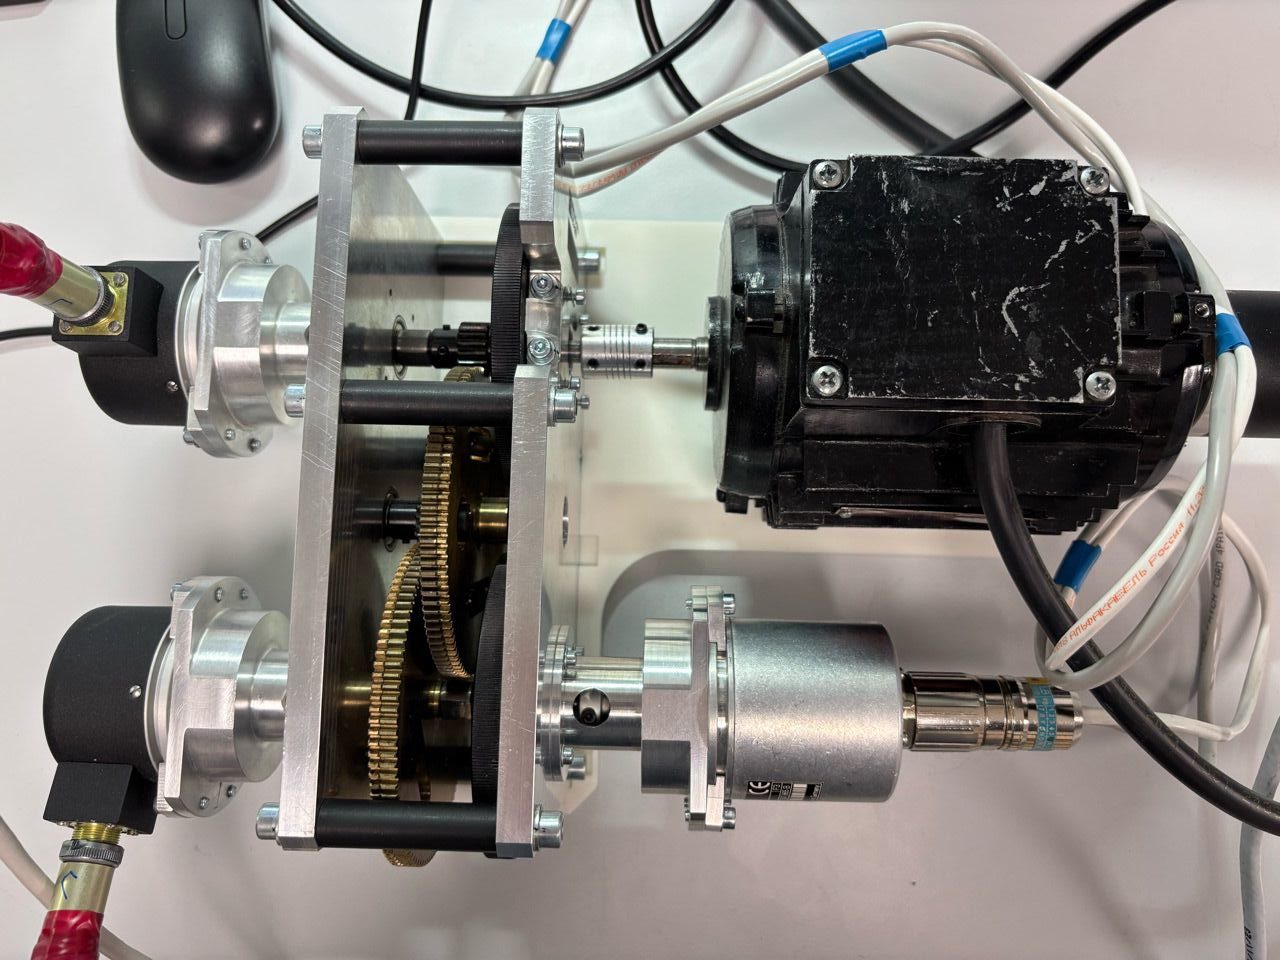
\includegraphics[width=\linewidth]{STND-01.jpg} 
    \label{STND01}
  \end{subfigure}
  \hfill
  \begin{subfigure}[b]{0.48\textwidth}
    \centering
    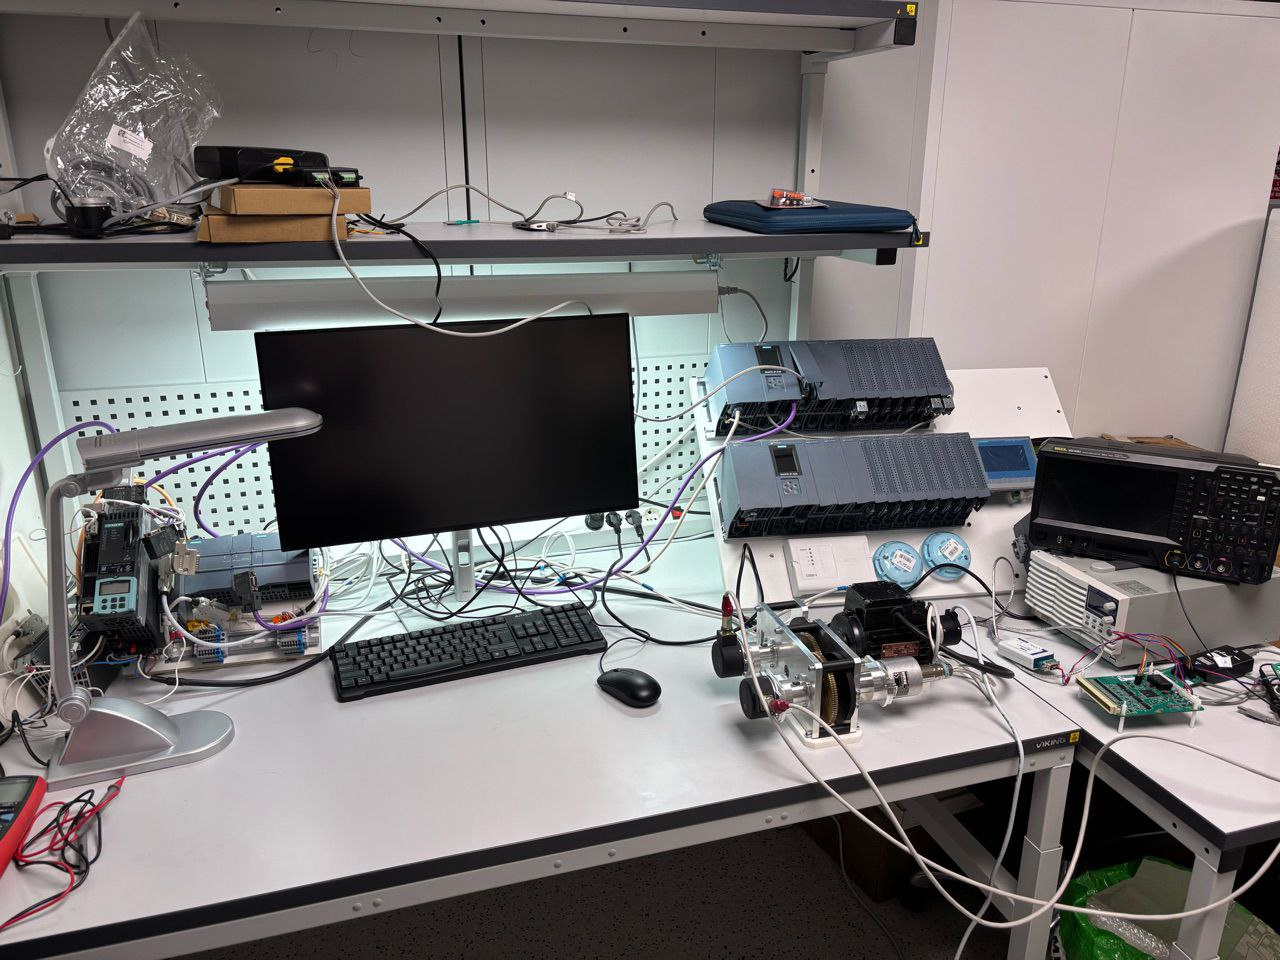
\includegraphics[width=\linewidth]{STND-02.jpg} 
    \label{STND02}
  \end{subfigure}

  \caption{Испытательный стенд}
  \label{STND-ISP} 
\end{figure}

\FloatBarrier

\section{Конечная точность следящей системы с астатизмом первого порядка}

В силу обратной связи, используемой в следящем алгоритме, погрешность в статическом позиционировании зависит от 
коэффициента $K_i$ \ref{eq:integration}. При выборе параметра, обеспечивающего достаточно быстрое схождение к норвому значению 
(экспериментально подобрано $K_i = 200$), погрещность в статическом режиме ничтожно мала. Было проведено исследование динамических характеристик 
при постоянной скорости вращения вала. Исследование включало в себя анализ погрешности слежения при постоянной скорости, максимально допустимой конструкцией
целевой антенной системы: $\omega = 30^\circ/\text{с}$. В эксперименте регистирировалась динамическая ошибка слежения 
$\delta(t) = \theta_{\text{зад}}(t) - \theta_{\text{изм}}(t)$.

\subsection{Программно-аппаратный комплекс}
Управление испытаниями осуществлялось специализированным ПО  \newline (LabVIEW 2021, National Instruments), обеспечивающим:
\begin{itemize}
    \item Генерацию управляющих воздействий на электропривод
    \item Сбор данных с частотой дискретизации 100 Гц
    \item Корреляционный анализ сигналов эталонного и тестируемого каналов
\end{itemize}


\section{Методология эксперимента}

\section{Результаты испытаний}

\subsection{Анализ динамической ошибки}
% \begin{figure}[h]
% \centering
% \includegraphics[width=0.9\textwidth]{error_distribution}
% \caption{Распределение динамической ошибки при $\omega=30^\circ$/c}
% \label{fig:error_dist}
% \end{figure}

Ключевые наблюдения по результатам эксперимента.
\begin{itemize}
\item В силу обратной связи система подавляет резкие отклонения.
\item В экспериментальных данных проявляется "инертность" обратной связи - накопленная ошибка влияет на новое измерение.

\end{itemize}

\section{Заключение}
Устройство удовлетворяет основному требованию. По результатам экспериментов в условиях постоянной угловой скорости вала, предельная ошибка 
системы постоянно оставалась в заданном диапазоне во время эксперимента ($2' \approx 0,033^\circ$). 


% (измеряем точность показаний схемы в установившемся режиме).

% \section{Конечная точность следящей системы с астатизмом второго порядка} % http://zrv.ivo.unn.ru/pages/vtp/6/6-1-sistemy-avtomaticheskogo-upravleniya.htm

